\documentclass[12pt,a4paper]{article}

% ── codificação e língua ───────────────────────────────────────────
\usepackage[utf8]{inputenc}
\usepackage[T1]{fontenc}
\usepackage[brazil]{babel}

% ── layout ────────────────────────────────────────────────────────
\usepackage[top=3cm,bottom=2cm,left=3cm,right=2cm]{geometry}
\usepackage{indentfirst}
\usepackage{setspace}
\onehalfspacing

% ── imagens ───────────────────────────────────────────────────────
\usepackage{graphicx}
\usepackage{float}

% ── tabelas ───────────────────────────────────────────────────────
\usepackage{booktabs}
\usepackage{array}

% ── código-fonte ──────────────────────────────────────────────────
\usepackage{listings}
\usepackage{xcolor}

\definecolor{kw}{RGB}{0,0,180}
\definecolor{cm}{RGB}{100,100,100}
\definecolor{st}{RGB}{160,0,0}
\definecolor{bg}{RGB}{250,250,250}
\definecolor{frame}{RGB}{200,200,200}

\lstdefinestyle{cstyle}{
    language=C,
    backgroundcolor=\color{bg},
    basicstyle=\ttfamily\small,
    keywordstyle=\color{kw}\bfseries,
    commentstyle=\color{cm}\itshape,
    stringstyle=\color{st},
    numbers=left,
    numberstyle=\tiny\color{cm},
    numbersep=10pt,
    frame=single,
    rulecolor=\color{frame},
    framerule=0.4pt,
    breaklines=true,
    breakatwhitespace=false,
    tabsize=4,
    showstringspaces=false,
    captionpos=b,
    xleftmargin=1.5em,
    literate=
        {ã}{{\~a}}1 {õ}{{\~o}}1 {â}{{\^a}}1 {ê}{{\^e}}1 {ô}{{\^o}}1
        {á}{{\'a}}1 {é}{{\'e}}1 {í}{{\'i}}1 {ó}{{\'o}}1 {ú}{{\'u}}1
        {Á}{{\'A}}1 {É}{{\'E}}1 {Í}{{\'I}}1 {Ó}{{\'O}}1 {Ú}{{\'U}}1
        {ç}{{\c{c}}}1 {Ç}{{\c{C}}}1,
}
\lstset{style=cstyle}

% ── cabeçalho/rodapé ──────────────────────────────────────────────
\usepackage{fancyhdr}
\pagestyle{fancy}
\fancyhf{}
\lhead{\footnotesize Algoritmos em Grafos -- PUC Goiás}
\rhead{\footnotesize Matheus Silva Pains}
\cfoot{\thepage}
\renewcommand{\headrulewidth}{0.4pt}

% ── hiperlinks ────────────────────────────────────────────────────
\usepackage[hidelinks]{hyperref}

% ── matemática ────────────────────────────────────────────────────
\usepackage{amsmath}

% ==================================================================
\begin{document}

% ── Capa ──────────────────────────────────────────────────────────
\begin{titlepage}
\centering
{\large \textbf{Pontifícia Universidade Católica de Goiás}}\\[0.3cm]
{\large Escola Politécnica e de Artes}\\[0.3cm]
{\large Ciência da Computação}\\[2.5cm]

{\Large \textbf{Algoritmos em Grafos}}\\[0.5cm]
{\large Busca em Largura (BFS) e Busca em Profundidade (DFS)}\\[2.5cm]

\begin{tabular}{rl}
\textbf{Aluno:}      & Matheus Silva Pains \\[4pt]
\textbf{Matrícula:}  & 2024.1.0028.0032-0  \\[4pt]
\textbf{Professor:}  & Dr.\ Robson Medrado de Oliveira \\[4pt]
\textbf{Disciplina:} & Algoritmos em Grafos \\[4pt]
\textbf{Prazo:}      & 29/05/2026
\end{tabular}

\vfill
{\large Goiânia, 2026}
\end{titlepage}

% ── Sumário ───────────────────────────────────────────────────────
\tableofcontents
\newpage

% ==================================================================
\section{Introdução}

Este relatório apresenta a implementação, em linguagem C, dos algoritmos de
Busca em Largura (\textit{Breadth-First Search} -- BFS) e de Busca em
Profundidade (\textit{Depth-First Search} -- DFS) aplicados a grafos não
direcionados.

O desenvolvimento utilizou o ambiente Visual Studio Code como editor e teve
como referência teórica o material disponibilizado pelo Prof.\ Dr.\ Robson
Medrado de Oliveira nas Aulas 10 e 11 da disciplina. Modelos de linguagem
natural foram utilizados como apoio para revisão e orientação da implementação.

% ==================================================================
\section{Motivação: por que buscar em grafos?}

Grafos são um dos modelos de dados mais versáteis da ciência da computação,
permitindo representar relações entre entidades em problemas como redes de
computadores, mapas, labirintos e redes sociais. A pergunta central que motiva
os algoritmos de busca pode ser formulada da seguinte forma:

\begin{quote}
\textit{Dado um grafo $G$ e um vértice inicial $s$, quais vértices podem
ser alcançados a partir de $s$?}
\end{quote}

Entre as aplicações práticas citadas no material de referência estão:
componentes conexas, detecção de ciclos, cálculo de distâncias entre vértices,
bipartição, identificação de arestas de corte e resolução de labirintos.

É importante distinguir grafos de árvores: enquanto árvores são grafos sem
ciclos e sem arestas paralelas --- admitindo percursos naturais como pré-ordem,
pós-ordem e por níveis ---, grafos gerais podem conter ciclos e múltiplos
caminhos entre dois vértices, o que torna necessária uma abordagem sistemática
de visitação.

% ==================================================================
\section{Algoritmo genérico de busca}

Ambas as implementações deste trabalho derivam de um mesmo algoritmo genérico
de busca. A ideia central consiste em construir, passo a passo, uma
\textbf{árvore de busca} $T$ dentro de $G$ a partir de um vértice inicial $s$.

A regra de expansão é: enquanto existir uma aresta $xy \in E(G)$ tal que
$x \in V(T)$ e $y \notin V(T)$, adicionam-se $y$ e a aresta $xy$ à árvore.
O algoritmo termina quando não há mais arestas desse tipo. Se ao final
$V(T) = V(G)$, o grafo é conexo; caso contrário, apenas a componente de $s$
foi alcançada.

Conforme destacado no material de referência, \textit{a árvore de busca pode
não ser única}, pois depende da ordem de escolha das arestas em cada iteração.
O que diferencia BFS de DFS é exatamente qual aresta (ou qual vértice) é
escolhido a cada passo --- e, consequentemente, qual estrutura de dados controla
essa escolha.

% ==================================================================
\section{Busca em Largura (BFS)}

\subsection{Descrição do algoritmo}

A BFS explora o grafo \textbf{por níveis}: primeiro visita todos os vizinhos
diretos de $s$, depois os vértices a distância 2, depois os a distância 3, e
assim por diante. O critério de escolha é sempre o vértice que foi alcançado
\textit{há mais tempo} entre os que ainda possuem vizinhos não visitados.

A estrutura de dados correspondente é a \textbf{fila} (FIFO ---
\textit{First In, First Out}).

O pseudocódigo seguido na implementação é o das Aulas 10 e 11:

\begin{verbatim}
BuscaLargura(G, s)
  s.visitado = 1
  cria fila vazia F
  Enfileira(F, s)
  enquanto F.tamanho > 0 faça
    u = Desenfileira(F)
    para todo v em N(u) faça
      se v.visitado = 0 então
        v.visitado    = 1
        v.predecessor = u
        Enfileira(F, v)
\end{verbatim}

\subsection{Implementação}

\lstinputlisting[
    caption={bfs.c -- Busca em Largura em grafo não direcionado},
    label={lst:bfs}
]{bfs.c}

\subsection{Resultados}

A Figura~\ref{fig:bfs} mostra dois testes executados com o mesmo grafo de
6 vértices e 7 arestas $\{(1,2),(1,3),(2,3),(2,4),(3,4),(3,5),(5,6)\}$,
variando apenas o vértice inicial.

\begin{figure}[H]
    \centering
    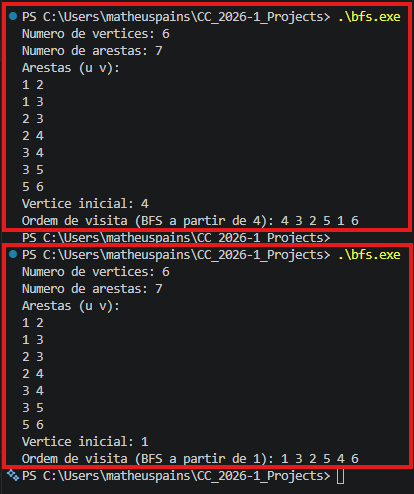
\includegraphics[width=0.65\textwidth]{bfs.png}
    \caption{Saída do programa BFS: vértice inicial 4 (acima) e vértice
    inicial 1 (abaixo).}
    \label{fig:bfs}
\end{figure}

\begin{center}
\begin{tabular}{ccc}
\toprule
\textbf{Vértice inicial} & \textbf{Ordem de visita} & \textbf{Níveis} \\
\midrule
4 & 4 3 2 5 1 6 & 0; 1; 2; 3 \\
1 & 1 3 2 5 4 6 & 0; 1; 2; 3 \\
\bottomrule
\end{tabular}
\end{center}

Como esperado, a ordem de visita muda com o vértice inicial, mas a lógica
de exploração por níveis é mantida em ambos os casos.

% ==================================================================
\section{Busca em Profundidade (DFS)}

\subsection{Descrição do algoritmo}

A DFS explora o grafo seguindo \textbf{um ramo o mais profundamente possível}
antes de retroceder (\textit{backtrack}). O critério de escolha é sempre o
vértice \textit{mais recentemente alcançado} que ainda possui vizinhos não
visitados.

A estrutura de dados correspondente é a \textbf{pilha} (LIFO ---
\textit{Last In, First Out}).

O pseudocódigo seguido na implementação é o das Aulas 10 e 11:

\begin{verbatim}
BuscaProfundidade(G, s)
  s.visitado = 1
  cria pilha vazia P
  Empilha(P, s)
  enquanto P.tamanho > 0 faça
    u = Consulta(P)
    se existe uv em E(G) com v.visitado = 0 então
      v.visitado    = 1
      v.predecessor = u
      Empilha(P, v)
    senão
      Desempilha(P)
\end{verbatim}

\subsection{Implementação}

\lstinputlisting[
    caption={dfs.c -- Busca em Profundidade em grafo não direcionado},
    label={lst:dfs}
]{dfs.c}

\subsection{Resultados}

A Figura~\ref{fig:dfs} mostra dois testes executados com o mesmo grafo
utilizado na BFS, variando o vértice inicial.

\begin{figure}[H]
    \centering
    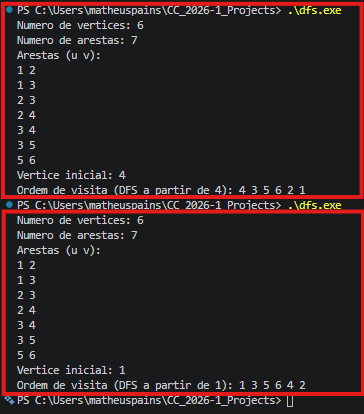
\includegraphics[width=0.60\textwidth]{dfs.png}
    \caption{Saída do programa DFS: vértice inicial 4 (acima) e vértice
    inicial 1 (abaixo).}
    \label{fig:dfs}
\end{figure}

\begin{center}
\begin{tabular}{cc}
\toprule
\textbf{Vértice inicial} & \textbf{Ordem de visita} \\
\midrule
4 & 4 3 5 6 2 1 \\
1 & 1 3 5 6 2 4 \\
\bottomrule
\end{tabular}
\end{center}

O comportamento de ``mergulho'' da DFS fica evidente: a partir do vértice
inicial, o algoritmo avança por um único caminho até não conseguir mais
prosseguir, e só então retrocede para tentar outro ramo.

% ==================================================================
\section{Comparação entre BFS e DFS}

A Tabela~\ref{tab:comp} resume as principais diferenças entre os dois
algoritmos.

\begin{table}[H]
\centering
\caption{Comparação entre BFS e DFS}
\label{tab:comp}
\begin{tabular}{lll}
\toprule
\textbf{Característica}     & \textbf{BFS}                    & \textbf{DFS} \\
\midrule
Estrutura de controle       & Fila (FIFO)                     & Pilha (LIFO) \\
Estratégia de exploração    & Por níveis                      & Por profundidade \\
Critério de escolha         & Mais antigo com vizinhos livres & Mais recente com vizinhos livres \\
Árvore gerada               & Árvore de largura               & Árvore de profundidade \\
Complexidade                & $O(V + E)$                      & $O(V + E)$ \\
Detecta ciclos?             & Sim (aresta entre visitados)    & Sim (aresta entre visitados) \\
\bottomrule
\end{tabular}
\end{table}

Ambos os algoritmos visitam cada vértice e cada aresta no máximo uma vez,
resultando na mesma complexidade assintótica $O(V + E)$. A diferença está
na \textit{ordem} em que os vértices são explorados, o que pode ser relevante
dependendo do problema a resolver --- BFS é preferível quando se busca o
caminho mais curto, enquanto DFS é base para algoritmos como detecção de
ciclos e ordenação topológica.

% ==================================================================
\section{Conclusão}

As implementações desenvolvidas seguem fielmente os pseudocódigos apresentados
nas Aulas 10 e 11, utilizando lista de adjacência para a representação do grafo,
fila circular estática para a BFS e pilha estática para a DFS. Os testes
realizados confirmaram o comportamento esperado de cada algoritmo: exploração
por níveis na BFS e exploração em profundidade na DFS. A variação do vértice
inicial alterou a ordem de visita em ambos os casos, o que é consistente com
a observação do material de referência de que a árvore de busca não é única.

\end{document}
